\documentclass[conference]{IEEEtran}
\IEEEoverridecommandlockouts
% The preceding line is only needed to identify funding in the first footnote. If that is unneeded, please comment it out.
\usepackage{cite}
\usepackage{amsmath,amssymb,amsfonts}
\usepackage{algorithmic}
\usepackage{graphicx}
\usepackage{textcomp}
\usepackage{xcolor}
\usepackage{float} % Add the float package for H specifier
\def\BibTeX{{\rm B\kern-.05em{\sc i\kern-.025em b}\kern-.08em
    T\kern-.1667em\lower.7ex\hbox{E}\kern-.125emX}}
\begin{document}
\onecolumn
\title{CSC 693 - HW 1 - LDA}
\author{Sahil Dhawan}
\maketitle
\section{Text Preprocessing}
\begin{enumerate}
    \item Split comments into sentences and report the average number of sentences per comment.\\
    \hspace{1cm}Average number of setences per comment = 10.704\\
    \item Do tokenization for the dataset and report the average number of tokens per comment.\\
    \hspace{1cm}Average number of words per comment = 152.028\\
    \item Without considering punctuation and stop words, how many words are in each comment on average?\\
    \hspace{1cm}Average number of words per comment, excluding stop words and punctuation = 100.982\\
    \item Try lemmatization and stemming for the database. What are the differences in the results based on your observation?\\
    \hspace{1cm}Average number of words per comment:
    \begin{itemize}
        \item Lemmatization\\
        \hspace{1cm}including stop words and punctuation: 144.087\\
        \hspace{1cm}excluding stop words and punctuation: 98.026
        \item Stemming\\
        \hspace{1cm}including stop words and punctuation: 140.205\\
        \hspace{1cm}excluding stop words and punctuation: 100.982
    \end{itemize}
    Lemmatization and Stemming create an almost equal amount of average words per comment, both including and excluding stop words and punctuation.
\end{enumerate}
\newpage
\section{Topic Modeling}
\begin{enumerate}
    \item Use the Latent Dirichlet Allocation (LDA) method to discover latent topics in the dataset. Try different numbers of topics for LDA. What number of topics do you think is more meaningful?\\
    \item Apply necessary text preprocessing techniques for the dataset. Are the topic modeling results better?\\
    \item If yes, you can use the preprocessed dataset for the following questions. With your topic model, what is the most relevant topic assigned to the document 0\_9.txt, 1\_7.txt, and 2\_9.txt? Do they make sense? Explain.\\
    \item Any method to better estimate the number of topics? Show it with your experiment.\\
    \item What are the possible limitations of the LDA topic model? (Do not just google it, try to show some of your understanding or explanation.)\\
    LDA is only as good as the preprocessing. It can attempt to identify topics in a comment or in a list of comments, but if the words do not have context with relation to the other high probability words, then the LDA topic probability densities will not give an accurate portrayal of the content of the data. For example, with 1 topic, without excluding stop words and punctuation, the most common tokens to appear are “the”, “a”, “,”, “.”, “to”, etc. but with exclusion, the most common tokens to appear are “film”, “movie”, “one”, “like”, “story”, “time”, etc. However, only the first two tokens are the most relevant to the dataset, while the rest are only tangentially related to movie reviews.
    
\end{enumerate}
\newpage
\section{Machine Learning}
\begin{figure}[H]
    \centering
    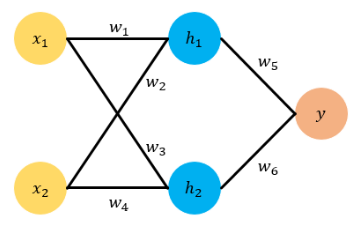
\includegraphics[scale=0.35]{HW 1 Neural Network Screenshot.png}
\end{figure}
Suppose we designed a neural network with the above structure with $x_1$ and $x_2$ as inputs and $y$ as output. $h_1$ and $h_2$ are simplified neurons without activation functions (or you can think the activation function is $y=x$). $w_1$ to $w_6$ are parameters. We have:
$$h_1 = w_1 * x_1 + w_2 * x_2$$
$$h_2 = w_3 * x_1 + w_4 * x_2$$
$$y = w_5 * h_1 + w_6 * h_2$$
We use the Backpropagation method to train this network, and let the error $E = 0.5(y-t)^2$ , where $t$ is the target (or label). If you are given the following dataset with one example:
\begin{table}[H]
    \centering
    \begin{tabular}{|c|c|c|c|}
     \hline
        Data & $x_1$ & $x_2$ & $t$ \\
     \hline
        Example 1 & 1 & 0.5 & 4 \\
     \hline
    \end{tabular}
\end{table}
and the initialized weights are: $w_1 = 0.5, w_2 = 1.5, w_3 = 2.3, w_4 = 3, w_5 = 1, w_6 = 1$
\begin{enumerate}
    \item What is the error after one epoch of feed-forward pass?\\
    $y = w_5(w_1 * x_1 + w_2 * x_2) + w_6 (w_3 * x_1 + w_4 * x_2)$\\
    $y = 1*(0.5*1+1.5*0.5)+1*(2.3*1+3*0.5) = 5.05$\\
    $E = 0.5 * (5.05-4)^2 = 0.55125$
    \item The error is not zero, so we need to update the weights following gradient descent. If we set the learning rate as $0.1$, what are the updated weights?\\
    $\gamma = 0.1$, $\frac{\partial E}{\partial y} = (y-t)$\\
    $y = w_5*h_1 + w_6*h_2 = w_5(w_1 * x_1 + w_2 * x_2) + w_6 (w_3 * x_1 + w_4 * x_2)$\\

	$\frac{\partial E}{\partial w_6}=\frac{\partial E}{\partial y} \times \frac{\partial y}{\partial w_6}=(y-t)*h_2=(y-t)*(w_3 * x_1 + w_4 * x_2)=(5.05-4)*(2.3*1+3*0.5)=3.99$\\
	$w_6 = 1 - \gamma * 3.99 = 1 - 0.1 * 3.99 = 0.601$\\
	
	$\frac{\partial E}{\partial w_5}=\frac{\partial E}{\partial y} \times \frac{\partial y}{\partial w_5}=(y-t)*h_1=(y-t)*(w_1 * x_1 + w_2 * x_2)=(5.05-4)*(0.5*1+1.5*0.5)=1.3125$\\
	$w_5=1 - \gamma * 1.3125 = 1 - 0.1 * 1.3125 = 0.86875$\\
	
	$\frac{\partial E}{\partial w_4}=\frac{\partial E}{\partial y} \times \frac{\partial y}{\partial w_4}=(y-t)*w_6 * x_2 = (5.05 - 4) * 1 * 0.5 = 0.525$\\
	$w_4=3-\gamma*0.525=3-0.1*0.525=2.9475$\\
	
	$\frac{\partial E}{\partial w_3}=\frac{\partial E}{\partial y} \times \frac{\partial y}{\partial w_3}=(y-t)*w_6*x_1 = (5.05-4)*1*1=1.05$\\
	$w_3=2.3-\gamma*1.05=2.3-0.1*1.05=2.195$\\

	$\frac{\partial E}{\partial w_2}=\frac{\partial E}{\partial y} \times \frac{\partial y}{\partial w_2}=(y-t)*w_5*x_2=(5.05-4)*1*0.5=0.525$\\
	$w_2=1.5-\gamma*0.525 = 1.5-0.1*0.525=1.4475$\\

	$\frac{\partial E}{\partial w_1}=\frac{\partial E}{\partial y} \times \frac{\partial y}{\partial w_1}=(y-t)*w_5*x_1=(5.05-4)*1*1=1.05$\\
	$w_1 = 0.5 - \gamma*1.05 = 0.5-0.1*1.05=0.395$\\
    \item With the updated weights, what is the new error? Is the error reduced?\\
    $y = w_5(w_1 * x_1 + w_2 * x_2) + w_6 (w_3 * x_1 + w_4 * x_2)$\\
	$y = 0.86875*(0.395*1+1.4475*0.5)+0.601*(2.195*1+2.9475*0.5) = 3.1768328125$\\
	$E = 0.5 * (3.1768328125 - 4)^2 = 0.33880210928$\\
	Yes, the error is reduced by 0.212447891.

\end{enumerate}

\end{document}
